\documentclass[first=purple,second=dblue,logo=redquo]{aaltoslides}

\usepackage[finnish]{babel}
\usepackage[utf8]{inputenc}
\usepackage[T1]{fontenc}
\usepackage{url}
\usepackage{lastpage}
\usepackage{hyperref}
\usepackage[style=finnish]{csquotes}
\usepackage{tikz}
\usetikzlibrary{positioning}
\usetikzlibrary{calc}
\usetikzlibrary{arrows}
\usetikzlibrary{decorations.pathmorphing,decorations.markings}
\usetikzlibrary{shapes}
\usetikzlibrary{patterns}
\usepackage{graphicx}
\PassOptionsToPackage{demo}{graphicx}

\newcommand\blfootnote[1]{%
  \begingroup
  \renewcommand\thefootnote{}\footnote{#1}%
  \addtocounter{footnote}{-1}%
  \endgroup
}

\usepackage[backend=biber,style=oscola]{biblatex}

\addbibresource{presisrefet.bib}

\title{Osaamisen kehityksen hallinta}

\author[M. Eloranta]{Miikka Eloranta}
\institute[AS]{Automaatio- ja systeemitekniikka\\
Sähkötekniikan korkeakoulu, Aalto-yliopisto}

\aaltofootertext{Osaamisen kehityksen hallinta}{20.03.2015}{\arabic{page}/\pageref{LastPage}\ }

\date{20.03.2015}

\begin{document}

\aaltotitleframe

\begin{frame}{Sisältö}
\begin{itemize}
\item Yleistä
\begin{itemize}
\item Työn sisällön kuvaus
\item Työn sisällön painopisteet ja taustat
\end{itemize}
\item Osaamiset
\begin{itemize}
\item Osaamisten ja niiden laadun määritys
\item Osaamisten jaottelu
\item T-malli
\end{itemize}
\item Kehittyminen
\begin{itemize}
\item Henkilöstön kehityssuunnitelmat
\item Yrityslaajuiset tavoitteet
\item Urakehitysmahdollisuudet
\end{itemize}
\item Keskitetyn osaamisten hallinnan hyödyt ja mahdollisuudet
\end{itemize}
\end{frame}

\begin{frame}{Yleistä}
\begin{itemize}
\item Osaamisen kehityksen keskitetty hallinta on ehdotonta etenkin suurissa ja nopeasti kasvavissa palveluyrityksissä
\begin{itemize}
\item Henkilöstön osaamisten tunteminen ulkomuistista mahdotonta
\end{itemize}
\item Työssä keskitytään ICT\footnote{\tiny{Tieto- ja viestintäteknologia (Information and Communications Technology)}}-palveluyrityksiin ja käytetyt menetelmät on määritelty niiden mukaisesti
\begin{itemize}
\item Osittain yleisemmän tason asiaa, joka soveltuu muillekin aloille
\end{itemize}
\item Työ keskittyy käytettyihin menetelmiin, kuvauksiin ja prosesseihin, ei kehitettyyn järjestelmään
\end{itemize}
\end{frame}

\begin{frame}{Osaamiset}
\begin{itemize}
\item Parhaat osoitukset osaamisesta ICT-maailmassa ovat sertifioitumiset ja referenssit
\begin{itemize}
\item Tarvitaan muitakin kuin teknologiaosaamisia \\ $\rightarrow$ Kaikkiin osaamisiin ei voi sertifioitua
\end{itemize}
\item Kilpailutuksessa asiakas huomioi myös kumppanit ja olemassaolevat asiakkuudet -- ennenkaikkea onko palveluyrityksellä jo saman toimialan asiakkaita \footcite{ICT-haasteet}
\item Saman koulutustaustan ihmiset voivat erota huomattavasti toisistaan \footcite{self-assessment_in_skill_measurement}
\end{itemize}
\end{frame}
\begin{frame}{Osaamisten määritys ja itsearviointi}
\begin{itemize}
\item Osaamisia on erityyppisiä ja kaikki halutaan saada merkittäviksi \\ $\rightarrow$ osaamiset on määritettävä irrallaan sertifioinneista (joskin nämä antavat osviittaa)
\item Osaamisen syvyys määritelty tasolla 1-5, joissa vaatimukset kullekin tasolle
\item Itsearvioinnin suosio perustuu nopeaan datankeruuseen \footcite{self-assessment_in_skill_measurement}
\begin{itemize}
\item Suuri määrä henkilöstöä $\rightarrow$ esimiesten aika ei riitä arviointiin
\item Myös epätäydellinen data on potentiaalisesti arvokasta
\item Esimiehen/erityisasiantuntijan arviolla voidaan korjata/vahvistaa arviointia
\end{itemize}
\end{itemize}
\end{frame}
\begin{frame}{Osaamisten T-malli}
\begin{tikzpicture}[remember picture,overlay]  
  \node [xshift=-0.35\textheight,yshift=-0.35\textheight] at (current page.north east)
    {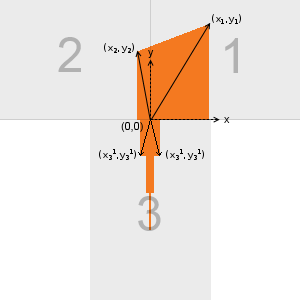
\includegraphics[width=0.45\textwidth]{T_drawing_logics2.png}};
\end{tikzpicture}
\begin{itemize}
\item Osaamiset jaotellaan kolmeen \\ osaamisalueeseen
\begin{enumerate}
\item Henkilökohtaiset kyvykkyydet
\item Organisaatio- ja toimialakohtaiset \\ osaamiset
\item Ammatilliset ja teknologiaosaamiset
\end{enumerate}
\item Piirtologiikka työroolikohtaiselle T:lle
\begin{itemize}
\item korkeus = osaamisten syvyys (taso)
\item leveys = osaamisten laajuus (lkm)
\item 1. ja 2. alueen tasoista lasketaan keskiarvo korkeudeksi
\item 3. alueen esitys ``vähintään tasolla x,'' josta johtuen porrastus
\item harmaa T, kun kaikki työroolin vaatimusosaamiset on tasolla 5
\end{itemize}
\end{itemize}
\end{frame}
\begin{frame}{Kehittyminen}
\begin{tikzpicture}[remember picture,overlay]  
  \node [xshift=-0.4\textheight,yshift=-0.3\textheight] at (current page.north east)
    {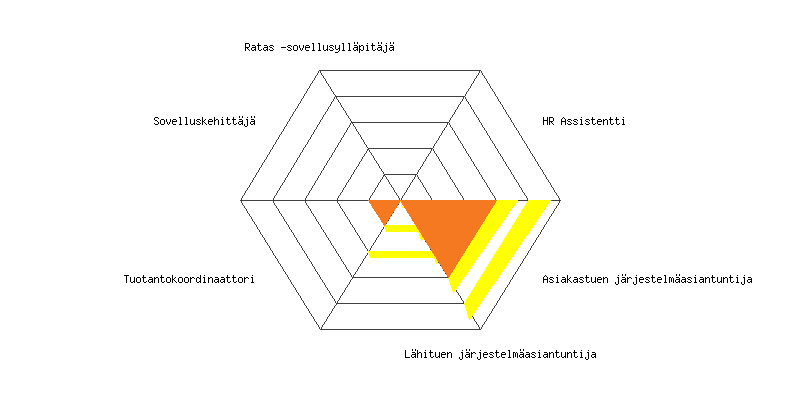
\includegraphics[width=.8\textwidth]{urapolkuPlot_tst_usr.png}};
\end{tikzpicture}
\begin{itemize}
\item Osaamisten kehittyminen \\ jatkuvaa henkilöstömuutosten, \\ teknologiakehitysten yms. \\ mukaisesti
\item Motivoitunut henkilöstö on kehittymisen \\ edellytys \\ $\rightarrow$ Henkilöstö itse vaikuttaa kehityssuunnitelmiinsa
\item Motivointina kehittymiseen urapolkujen esitys
\begin{itemize}
\item Miten henkilö voisi edetä urallansa muihin rooleihin
\item Oranssilla nykyrooli ja sen taso, harmaalla vaatimusten täyttymisaste
\end{itemize}
\end{itemize}
\end{frame}
\begin{frame}{Yritystason tavoitteet}
\begin{itemize}
\item Johdon määrittämät tavoitteet koko yritykselle
\begin{itemize}
\item Konkretisoituvat laskeuduttaessa organisaatioportaittain alaspäin
\item Voi olla määritelty myös henkilöstön kehittymissuunnitelmien perusteella!
\end{itemize}
\end{itemize}
\begin{figure}
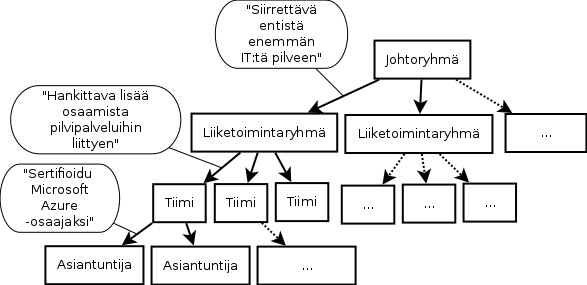
\includegraphics[width=.8\textwidth]{tavoitesample.png}
\end{figure}
\end{frame}
\begin{frame}{Keskitetty hallinta}
\begin{itemize}
\item Haasteet:
\begin{itemize}
\item Käytön oltava aktiivista jokaisen työntekijän osalta, jotta koko yrityksen laajuinen osaamisraportointi luotettavaa
\item Jatkokehitysideoita paljon $\rightarrow$ karsinta ja priorisointi
\end{itemize}
\item Hyödyt ja mahdollisuudet:
\begin{itemize}
\item Kehittymisen seuranta ja osaamisraportointi helpottuu ja nopeutuu huomattavasti \\ $\rightarrow$ HRM\footnote{\tiny{Henkilöstöhallinto (Human Resource Management)}}-tarpeiden nopea yleiskatsaus
\item Rajapinnoilla ja integroinneilla voidaan hyödyntää myös mm. HR-järjestelmän dataa \\ $\rightarrow$ Integraatioita hyödyntämällä ja toiminnallisuuksien lisäyksillä suuri määrä jatkokehitysmahdollisuuksia
\end{itemize}
\end{itemize}
\end{frame}
{
\usebackgroundtemplate{%
  \vbox to \paperheight{\vfil\hbox to \paperwidth{\hfil
\includegraphics[width=1.5in]{akatemia-logo.png}\hfil}\vfil}
}
\begin{frame}{Malli-CV}
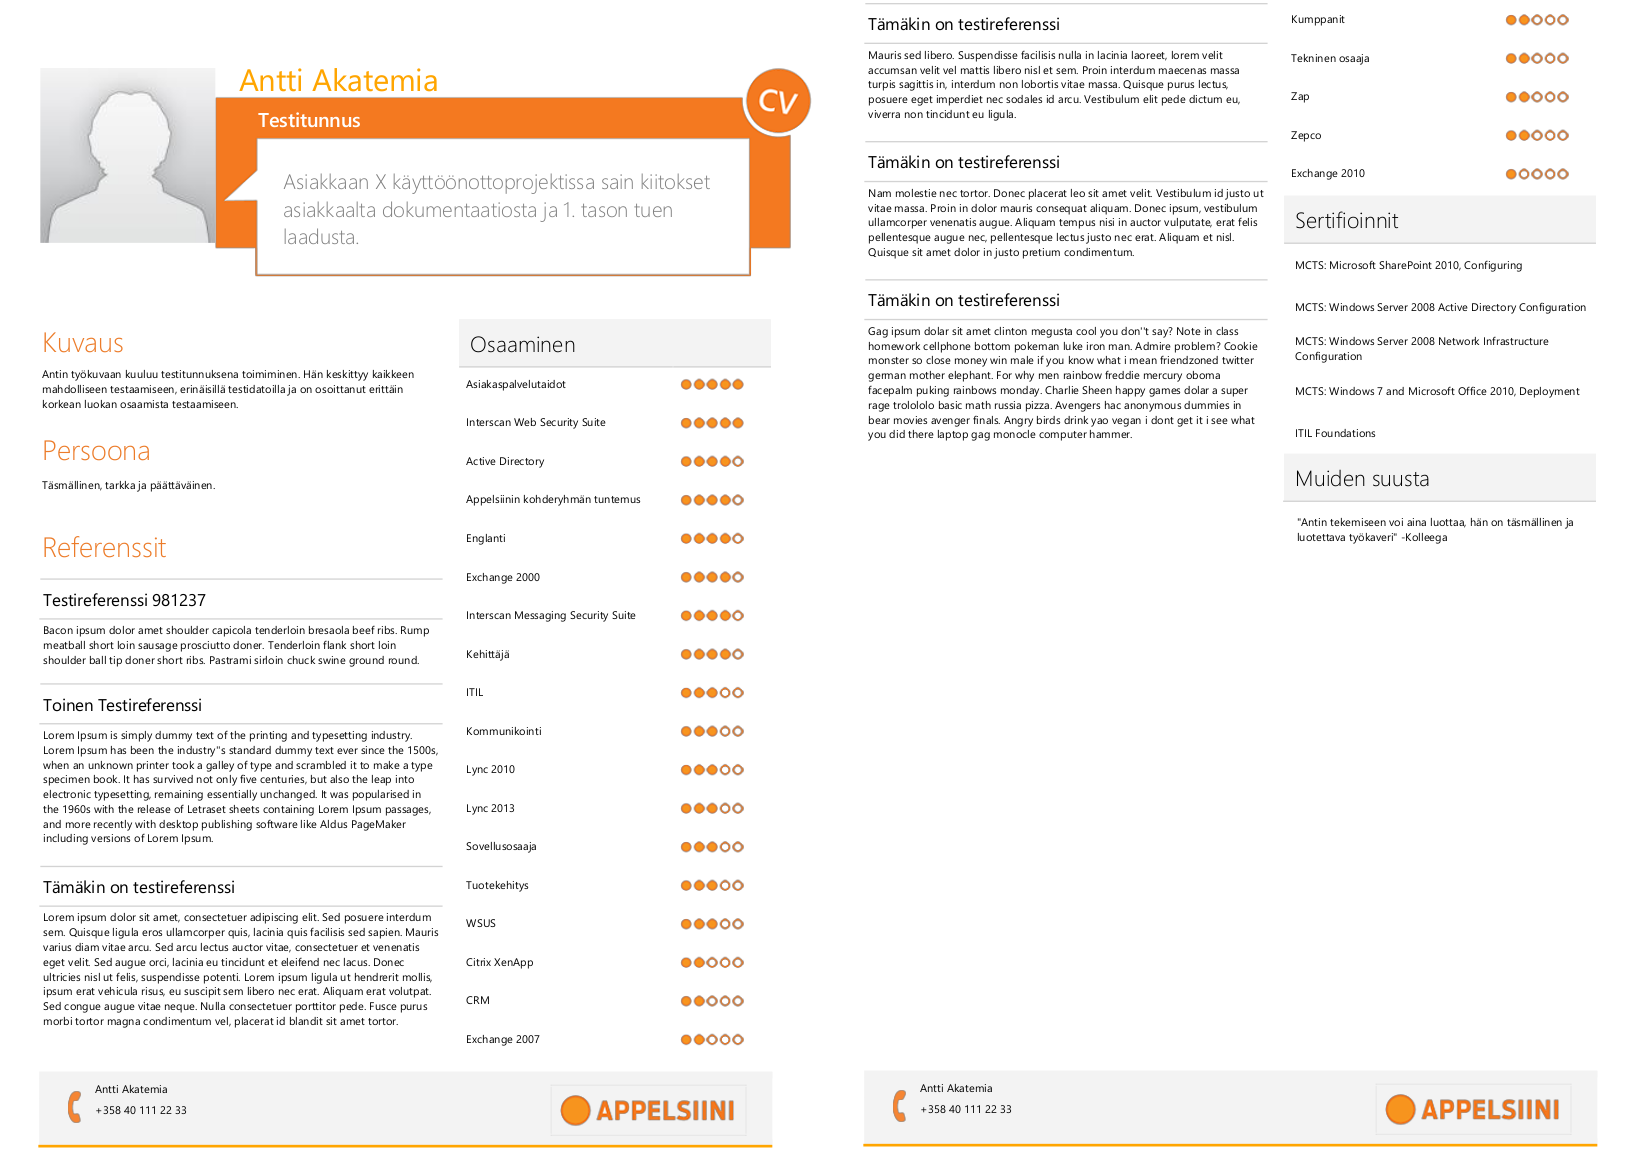
\includegraphics[width=\textwidth]{Akatemia_sampleCV.png} \blfootnote{\tiny{Järjestelmän käyttäjätiedot integroitu Microsoft Active Directory:sta ja CV luotu Microsoft SQL Server Reporting Services -raporttipohjalle järjestelmän datasta.}}
\end{frame}
\begin{frame}{?}
\begin{center}
Kysymyksiä, kommentteja?
\end{center}
\end{frame}
}
%% Lähdeluettelo
%\begin{frame}{Viitteet}
%\printbibliography
%\end{frame}
\end{document}
